\chapter{Implementation}
\label{chapter:implementation}
  This chapter will discuss the specific implementation details for both project components: the Haar Engine and Haar demonstration application.

  % Chapter structure

  \section{Hosting}
    The software components for this project were hosted on a public web server for demonstration and testing purposes. There are a large number of hosting solutions available; in this case, a Virtual Private Server (VPS) was chosen. A VPS was chosen over competing solutions (such as a Platform as a Service like Heroku) because its offers complete control over installed software and their configuration. The VPS chosen is also scalable, meaning that it can be configured with more or fewer system resources in response to demand.

    The VPS was installed with the open source Debian 8 Linux operating system. Debian was created in 1993 making it one of the oldest Linux distributions available; the open source community has been actively patching bugs and implementing new features ever since. Debian comes with very little pre-installed but it does have access to access to the Aptitude package registry, from which many popular applications can be installed. These characteristics make Debian the ideal foundation for a web server.

    Very little configuration was made to the VPS itself. Beyond some basic user and SSH configuration, the only additional packages required were Uncomplicated Firewall (UFW) and the Docker Cloud agent. UFW was used to create a strict firewall policy in order to protect the server for unauthorised access. Section \ref{section:docker} (Docker) explained that Docker images can be compared to virtual machines. Since Docker images contain all software which they require to run, nothing extra must be installed on the host. The Docker Cloud agent is simply used to connect the VPS to the Docker Cloud deployment service.

    A reverse proxy was used to expose Docker containers to the Internet. The Nginx web server was chosen for this purpose because it is event-based (as opposed to process-based like the Apache web server) which makes it more efficient at handling concurrent connections. Nginx also has great first-party support for proxy and caching functionality. The reverse proxy had two main responsibilities: TLS and HTTP/2 termination. These enable the API and dashboard to be served over a secure HTTPS tunnel and for web browsers to leverage performance-enhancing features. Figure x.x illustrates this implementation. In keeping with the development practices used, the Nginx reverse proxy was also wrapped up into a Docker image.

    \begin{figure}
      \centering
      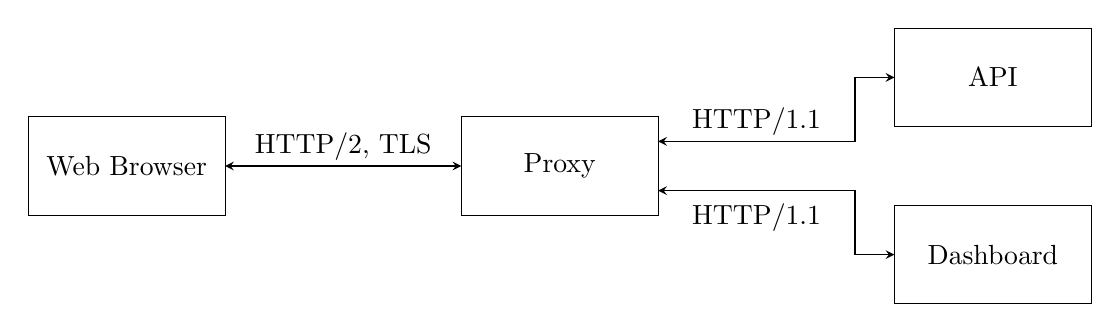
\begin{tikzpicture}
        \draw (0,1.125) rectangle (2.5, 2.375) node[midway] {Web Browser};
        \node[align=center] at (4,2) {HTTP/2, TLS};
        \draw[<->, >=stealth] (2.5,1.75) -- (5.5,1.75);

        \draw (5.5,1.125) rectangle (8, 2.375) node[midway] {Proxy};

        \draw (11,2.25) rectangle (13.5, 3.5) node[midway] {API};
        \node[align=center] at (9.25, 2.3125) {HTTP/1.1};
        \draw[<->, >=stealth] (8,2.0625) -- (10.5,2.0625) -- (10.5,2.875) -- (11,2.875);

        \draw (11,0) rectangle (13.5, 1.25) node[midway] {Dashboard};
        \node[align=center] at (9.25, 1.1) {HTTP/1.1};
        \draw[<->, >=stealth] (8,1.4375) -- (10.5,1.4375) -- (10.5,0.625) -- (11,0.625);
      \end{tikzpicture}
      \caption{Web server request flow}
      \label{figure:reverse-proxy}
    \end{figure}

  \section{Haar Engine}
    % purpose
    % how to use it

    \subsection{Node.js and npm}
      Chapter \ref{chapter:design} (Design) identified Node.js as the most suitable programming environment for the Haar Engine. There are a number of characteristics  about Node.js which have been employed in this implementation, including: functional composition, package managment and incremental standard support.

      The development ethos of the Node.js and wider JavaScript community is to embrace the functional programming paradigm and to compose applications with increasingly specific modules. To support this ethos, Node Package Manager (npm) is used as a global open source registry of reusable modules. To be compatible with this registry, any given module must provide a `package.json' file in the project root. This file includes (amongst other options): a version number; author details; any npm dependencies and lifecycle commands like start or test.

      Haar Engine employed the features of npm to aid development and to encourage extensibility. In particular, a number of open source npm packages were used for this project and were specified in the `package.json' file. In accordance with the professional considerations described in Chapter \ref{chapter:profession-considerations}, full credit has been given to the authors of these projects in Appendix \ref{chapter:credits}. Additionally, the Haar Engine itself can be included as a project dependency since it adheres to the requirements of npm. This is exactly the purpose of this software component---to be an extensible framework to build from.

      One final detail regarding Node.js is the version of JavaScript used. JavaScript itself is an implementation of a standard: ECMAScript. The latest version of ECMAScript (ES2015) was ratified in June 2015 \citep{es2015} and as a result, new language features and syntax are slowly being implemented by JavaScript engines. Embracing cutting-edge features for client-side JavaScript has historically been troublesome due to the number of available browsers, however this problem does not exist in Node.js. Developers of server-side applications can support whichever language features that are installed on the server. Given this opportunity, Haar Engine has been implemented using native ES2015 syntax. This requirement has been specified in `package.json'.

    \subsection{MongoDB Database}
      The main goal of the Haar Engine is to provide an extensible framework for IoT applications. One of the key features in support of this was a database connector layer which would enable developers to support a variety of database types. As the implementation progressed, it became clear that this feature would introduce too much complexity, given the constraints of this project. Rather than implementing a layer which supported a variety of strict database schemas, only one, highly flexible database solution is supported. This method resolved the extensibilty requirement from a different angle.

      The NoSQL database `MongoDB' was chosen for a number of reasons. First of all, the flexibility of a NoSQL versus a relational SQL database allows the schema to be very dynamic and to change with the data. This makes it simpler for a developer to add new data structures. In comparison, to modify an SQL database the developer would have to first update the database schema using a Data Definition Language (DDL). MongoDB was selected from the avaiable NoSQL database solutions because its data structure is based on JavaScript Object Notation (JSON). This makes it easy to interface with the Node.js application code. There are also a number of helper packages available for Node.js (including Mongoose which is described below).

    \subsection{MVC Architecture}
      A Model-View-Controller (MVC) architecture formed the basis of the Haar Engine implementation. This architecture is widely employed in web application development. \citet{google-mvc} state that ``MVC offers architectural benefits over standard JavaScript'' and go on to explain that an MVC architecture helps to develop organised, more maintainable code.

      Models were implemented using the Mongoose Object Data Mapping (ODM) package. As has been explained, the underlying NoSQL database was chosen because of its superior flexibility. However, this flexibility can introduce its own challanges in maintaining a standardised schema. The Mongoose package helps to control the flexbility through schema definitions and field validation. Mongoose also adds additional app-layer tools on top of MongoDB, such as document population (expanding child documents based on an ID) and virtual getters (computed fields). Document population in particular was used for the Haar Engine.

      The Express web application framework was used to implement controllers. These controllers represent the RESTful Data Access API endpoints. Listing \ref{express-route} illustrates an example Express controller, comprising of a URL structure and a handler. The URL structure can contain static segments like `/users' or dynamic tokens like `/:user' (which would then be made available to the handler). Each controller handler is passed `req' and `res' objects. As would be expected, the `req' object provides information about the current request (such as form data) and the `res' object is used to handle the response.

      \begin{lstlisting}[caption=An example Express controller,
        label=express-route,
        captionpos=b,
        numbers=none,
        frame=single,
        float]
const express = require(`express');
const router = express.Router();

router.get(`/users/:user', (req, res) => {
  
  // Perform controller action
  // URL token is available from `req.params.user'
  // Response is sent with `res.json({data: 'The Data'})'

});
      \end{lstlisting}

      The Data Access API returns JSON strings and these are considered views of the system. A standard response format was created in order to maintain consistency for API requests. The possible keys of the JSON response is illustrated in Listing \ref{json-response}.
      
      \begin{lstlisting}[caption=The standard JSON format,
        label=json-response,
        captionpos=b,
        numbers=none,
        frame=single,
        float]
{
  ``status":"success",
  ``meta": {
    ``message": ``A response message",
    ``validation": {
      ``errors": {
        ``field": ``Validation error"
      },
      ``values" {
        ``field": ``Existing value"
      }
    },
    ``paginate": {
      ``total": 22,
      ``pages": 2,
      ``currentPage": 1,
      ``previousPage": null,
      ``nextPage": 2
    }
  },
  ``data": [
    {
      ``field1": ``Field1 Data",
      ``field2": ``Field2 Data"
    },

    ...

  ]
}
      \end{lstlisting}
    \subsection{Real-Time}
      The \textit{raison d'etre} of this project is to implement real-time, bidirectional machine-to-machine communication. This was to be implemented as a WebSocket service managed by the Socket.io package. The implementation progressed as planned until Haar Engine began to expose limitations of Socket.io---or rather, the capability of Socket.io was being stretched in directions it was not designed for. The issues stemmed from the publish/subscribe model being applied to Socket.io; device and user authentication was not feasible using the package's built-in namespace and room features.

      An alternative package called Primus was found to be more suitable. Primus supports a number of lower-level communication libraries (including Engine.io, the library which Socket.io is built on) and is ultimately more flexible. Primus also exposes a plugin architecture which allows third-party developers to implement new features. Two such plugins were included to provide the desired features: Primus Rooms and Primus Responder. Primus Rooms supports a room hierarchy (like `subscribe:sensor:\textit{device}') which mimics the hierarchical structure of MQTT topics. Also, Primus does not send acknowledgement messages by default; Primus Responder provides this feature.

      The Primus Responder plugin demonstrates both the fragility and strengths of Open Source Software. When initially building Primus into the Haar Engine, Primus Responder failed to execute. Due to updates in one of its dependencies, Primus Responder had developed a software bug. Whilst waiting for the package author to implement a fix, a `fork' of the project was made for use in the Haar Engine. The fork fixed the bug and allowed implementation to continue.

      The operation of the real-time connection manager successfully supports publish/subscribe behaviour. Listing \ref{realtime-index} illustrates an important excerpt from the file `/lib/realtime/index.js'. The excerpt shows the declaration of an array of handler functions. When a new message is received by the connection manager, the received room option is tested against the regular expressions defined in each array item. If the room matches, its sibling key `handler' is executed. For example, a message sent to the room `input:stream:a1b2c3d4e5f6g7h8i9j0k1l2' will be subscribed to data events for the device with ID `a1b2c3d4e5f6g7h8i9j0k1l2' (pending authentication).

      \begin{lstlisting}[caption=Excerpt from `/lib/realtime/index.js',
        label=realtime-index,
        captionpos=b,
        numbers=left,
        frame=single,
        firstnumber=10,
        float]
const handlers = [
  {
    room: /^(input):(add)$/,
    action: 'publish',
    handler: input.publish,
  },
  {
    room: /^(input):(stream):([a-fA-F0-9]{24})$/,
    action: 'subscribe',
    handler: input.subscribe,
  },
  {
    room: /^(input):(stream):([a-fA-F0-9]{24})$/,
    action: 'unsubscribe',
    handler: input.unsubscribe,
  },
  {
    room: /^(output):(stream):([a-fA-F0-9]{24})$/,
    action: 'subscribe',
    handler: output.subscribe,
  },
  {
    room: /^(output):(stream):([a-fA-F0-9]{24})$/,
    action: 'unsubscribe',
    handler: output.unsubscribe,
  },
];
      \end{lstlisting}

      The operation of the `publish' action also merits further discussion. This represents the stream processor component that was discussed in Chapter \ref{chapter:design} (Design). After the datapoint has been persisted to the database, it is necessary to execute any active rules. Rules for the Haar Engine are a complete JavaScript script with access to standard runtime functions. It is dangerous and often discouraged to accept and execute untrusted third-party code, but this is necessary for this use-case.

      A sandboxed runtime environment is used to safely execute rules. This feature is provided by a native Node.js module called `vm'. It executes the user-provided rule in a seperate Google V8 engine instance and then returns the result. A side-effect of using this module is that it also catches syntax errors in the rule---a capability which has been used when validating new or updated rules.

    \subsection{Security}
      Sound application security is the sum of many parts. It is the responsibility of this software component to enforce user authentication and authorisation, as well as protecting access to supporting software like backing databases. The security of Haar Engine has been hardened through the careful consideration and implementation of: configuration variables, strong password hashing, token-based authentication, application middleware and Cross-Origin Resource Sharing (CORS).

      Haar Engine must be provided configuration settings in order to execute. These configuration settings contain, amongst other things, the database server URL and access credentials. The Haar Engine delegates the responsibility of managing these credentials to the developer, but they are encouraged to use environment variables. Environment variables have local scope meaning that they are available only to the process in which they were set \citet{env-vars}. This is ideal behaviour for confidential credentials and ensures that they are available to software which requires them.

      Strong password hashing is used to store user passwords. Best practices can be used to secure the servers running database applications, however if the database is accessed by a malicious actor additional safeguards must be in place to protect sensitive data. Hashing is a process which irreversibly obscures data. A number of algorithms exist for this purpose such as MD5 and the SHA family of algorithms, however bcrypt is currently considered the \textit{de facto} standard for password hashing \citet{hashing-algorithms}. Bcrypt is particularly strong due to its memory requirements and due to this, it would take too long for a malicious actor to crack. The bcrypt hashing algorithm has been implemented to securely store passwords.

      JSON Web Tokens (JWT) are used to authenticate API requests. The Data Access API has been implemented using the RESTful architecture and is therefore stateless---every request sent to the API must contain all required information. The process begins when a user authenticates using their username and password combination. If successful, the API will return a signed JSON Web Token, containing information about the user and an expiration date. For every subsequent request to the API the token must also be sent in order to be granted access. When compared to stateful server-side sessions, the use of stateless tokens is more secure because it protects against Cross-Site Request Forgery (CSRF) attacks.

      Haar Engine uses middleware to ensure that user authentication is applied consistently. Both Express (used for Data Access API) and Primus (used for Real-Time Event API) support the notion of middleware---functions which are executed in series and can stop a request or pass it onto the next middleware handler. Authentication middleware interrogates the request for a valid JSON Web Token. If the JWT is invalid or does not exist, the middleware will stop the request and prevent access.

      % CSRF
        % CORS

    \subsection{Testing}
      Extensive testing was carried out during the implementation of the Haar Engine. The purpose of the tests was to ensure that code was of a certain quality and that the application functioned as expected. Testing existed in three forms: code quality assertion, unit testing and acceptance testing.

      The pre-commit hook as describe in Section \ref{section:pre-commit-hook} was used to ensure good code quality. JavaScript is a very flexible language and the same problem can be solved with many different methods. Over time, the community has learnt from mistakes to develop widely-accepted best practices. A tool called ESLint tests JavaScript files against a pre-defined list of rules, flagging syntax or conventions which are considered poor practice. For this project, ESLint is triggered by the pre-commit hook in Git VCS and prevents poor code from being committed to the database.

      A suite of 96 unit tests was developed to ensure that system components functioned correctly. Testing dynamic web applications such as the Haar Engine is made difficult due to the additional dependencies which they require, such as databases. One solution to test database-dependent code is to mock queries with dummy data structures rather than a live database connection. This is however not a true representation of the system. Since Docker was being used to enforce a consistent development environment, it could also be used to run the unit tests against a live database. For the purposes of testing, a test database was seeded with example data.

      The Data Access API is a main system component and was also challenging to test effectively. In order to test the execution of the API, an HTTP request must be made to the controller and the response body interrogated. An npm package called Supertest was used for this purpose. It allows HTTP endpoints to be tested programatically, interrogating the response for specific headers and body properties.

      The final category of testing performed on the Haar Engine is acceptance testing. The purpose of acceptance testing is to compare the finished product against requirements specifications defined. The results of this testing can be found in Appendix \ref{haar-engine-acceptance-tests} and will be discussed in further detail as part of the next chapter.

  \section{Haar API}
    The second software component produced for this project is Haar, a demonstration implementation of Haar Engine. The main purpose of this demonstration application is to validate the design decisions and to show, by example, that the theory behind this IoT framework works. The implementation of Haar has been split further into four sub-components: API, Dashboard, Bridge and Nodes.

    Haar API is the actual implementation of Haar Engine. Since the aim of Haar Engine is to provide a starting point for an IoT application, the sole purpose of Haar API is to bootstrap the framework and show that it can be included as a project dependency. Quite simply, Haar API includes Haar Engine as a dependency from Github.

  \section{Haar Dashboard}
    Haar Dashboard is a web-based user interface built on top of the suite of Haar Engine APIs. It utilises both the Data Access API to configure system settings and the Real-Time API to subscribe to live data events. Whilst not necessary for the operation of the underlying IoT framework, the Haar Dashboard UI makes configuring devices simple and illustrates how a viable consumer solution might work.

    Section \ref{section:front-end-application} (Front-End Application) briefly discussed the challenges facing this user interface. In particular, certain components of the user interface must react to real-time events. The solution selected to address the challenges was a single-page JavaScript web application (SPA). The following section will describe the implementation of this technique, how it satisfies design goals and how it addresses these challenges.

    \subsection{JavaScript Application Framework}
      There are a wide variety of JavaScript frameworks which aid in the development of single-page web applications. While these frameworks differ in what problems they solve and how they solve them, they share some common characteristics.

      The general aim of a single-page web application is to create a more responsive and user friendly interface, much like would be experienced with a desktop application. This is achieved through the use of asynchronous AJAX requests; rather than navigate to new web pages, the correct data is requested and loaded into the existing web page. This also requires all of the application logic to be retrieved with the initial page request. Since the web page will not be reloaded, this makes it ideal for opening and maintaining the WebSocket connection required for this component.

      Single-page web applications also introduce new challenges. One of the hurdles to overcome is the inital load time. Since all of the application logic must be loaded before the web app can be used, users can experience long initial delays. There are also accessibility and usability challenges due to how the content is loaded. The initial HTML response from the server will be empty or will contain very basic content because content is loaded dynamically by the application. This means that search engine crawlers or users without JavaScript enabled canot view the web page content.

      The features offered by the React JavaScript framework implemented for this project go some distance in resolving these challenges. React is a project developed by software engineers at Facebook. It is based on the concept of a tree composable components, where a single component encapsulates all of the logic which it requires to execute, including CSS styles. What is most clever about React is its use of a virtual Document Object Model (DOM). React will first build up the tree of components using this virtual DOM before comparing it against the actual DOM. If anything has changed, React will only update the affected components.

      React can use this virtual DOM to render web pages server-side. React will build up a webpage and send it as the body of an HTML response. Once the client-side code has loaded, React will then bootstrap the application based on the existing body. This concept is known as Isomorphic or Universal JavaScript. Since an HTML body is returned, most features of an application can be used straight away. Search engine crawlers and accessibility tools can also parse the body, solving the challenges traditional single-page JavaScript web applications.

      As was discussed for the implementation of Haar Engine, the latest features of JavaScript are defined in the ECMAScript 2015 standard. Some web browsers can be slow to implement new features whilst other, older browsers may not implement them at all. This is a headache for developers; new features and syntax might solve problems in a more effective way, but they may not be supported by every target browser. This is where so-called front-end tooling is used. A variety of tools exist to convert new, uncompatible syntax into older, widely supported syntax. In particular a package called Babel has been used in this project to compile ES2015 syntax into ECMAScript 5 compatible code, meaning it can be run in all modern browsers. Additionally, a tool called Webpack has been used to package server-side JavaScript modules for use within the browser.

    \subsection{Data Management}
      The features which React provide solve half of the front-end engineering problem. React defines how data is manipulated and displayed, but it does not specify how the data itself is managed. For that reason, Facebook have also invented a development pattern called Flux. Flux provides a strict method by which data is added or updated then introduced to the React component tree. The fundamental rule of Flux is that the data flow is unidirectional; that is, data cannot be mutated directly but rather through a pre-defined process. Figure \ref{figure:flux-flow} illustrates this process. Redux has become the \textit{de facto} implementation of this pattern and will be used in this project.

      \begin{figure}
        \centering
        \begin{tikzpicture}
          \draw (0,0) rectangle (2.5, 1.25);
          \node[align=center] at (1.25,0.625) {Action};
          \draw[->, >=stealth] (2.5,0.625) -- (3.5,0.625);

          \draw[<-, >=stealth] (4.75,1.25) -- (4.75,2.875) -- (7,2.875);
          \draw (7,2.25) rectangle (9.5, 3.5);
          \node[align=center] at (8.25,2.875) {Action};
          \draw[<-, >=stealth] (9.5,2.875) -- (11.75,2.875) -- (11.75,1.25);

          \draw (3.5,0) rectangle (6, 1.25);
          \node[align=center] at (4.75,0.625) {Dispatcher};
          \draw[->, >=stealth] (6,0.625) -- (7,0.625);

          \draw (7,0) rectangle (9.5, 1.25);
          \node[align=center] at (8.25,0.625) {Store};
          \draw[->, >=stealth] (9.5,0.625) -- (10.5,0.625);

          \draw (10.5,0) rectangle (13, 1.25);
          \node[align=center] at (11.75,0.625) {View};
        \end{tikzpicture}
      \caption{Data flow in a Flux React application}\label{figure:flux-flow}
      \end{figure}

      Redux makes managing complex data more simple and this has proven particularly effective when managing forms. There are many forms used by Haar Dashboard to collect data from the user. Some forms, such as when adding a new user, have simple fields which can be represented by standard HTML constructs. However there is a requirement to manage more complex form data, such as an array of data descriptors for the device types. It would be very easy for the JavaScript code managing this to become unweildy. However, the structure which Redux gives to data makes mirroring the database model structure straightforward. Figure x.x. illustrates that objects and arrays have been modelled in HTML forms using this technique.

      \begin{figure}
        \centering
          \begin{tikzpicture}
            \node[inner sep=0pt] at (0,0)
              {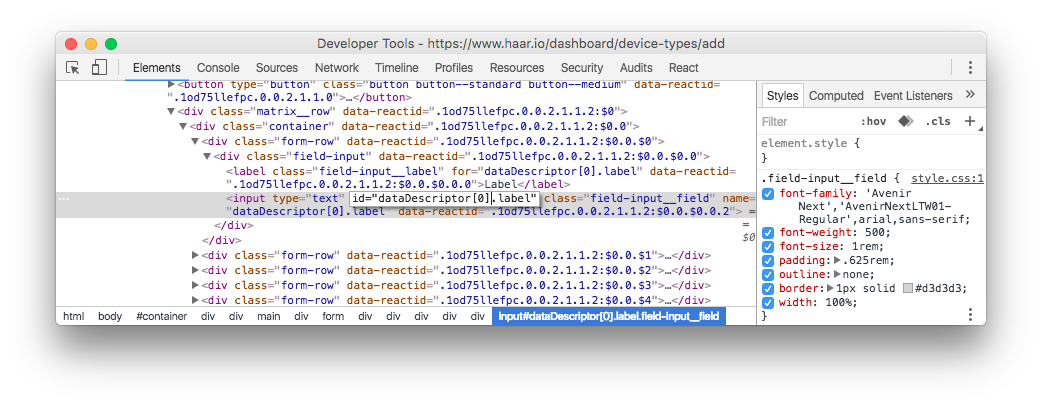
\includegraphics[width=\textwidth]{assets/form-array.png}};
          \end{tikzpicture}
        \caption{Complex data structures are easily managed with Redux}
        \label{figure:form-array}
      \end{figure}

    \subsection{Real-time}
      One of the most interesting features which Haar Dashboard demonstrates is its real-time event handling. Most of the front-end implementation details have been chosen in order to make real-time interactivity feasible. In particular, the single-page application architecture makes it possible to maintain a bidirectional WebSocket connection; the virtual DOM feature of React makes updating the web page fast and efficient, and finally, the data managament offered by the Flux pattern ensures that data updates can be controlled. When combined, these three characteristics not only make real-time connectivity possible, but they make it efficient and maintainable.

      The Primus package used to managed WebSocket connections in Haar Engine also generates a client-side library. This library is used in Haar Dashboard to negotiate and maintain the actual WebSocket tunnel. Once the connection has been opened, it is then the responsibility of the Redux actions to authenticate the user and to subscribe/unsubscribe to the appropriate sensor event streams. When a new sensor event is received, a Redux action will be dispatched and handled appropriately. This functionality can be demonsrated with the `live data' feature of sensor data pages.

    \subsection{Security}
      Haar Dashboard has its own role to play in the security of the complete application. First of all, the user interface must only be accessible to users with correct and authenticated credentials as proven by a valid JWT token. Although Haar API will not return application data without the presence of a valid token, Haar Dashboard should take responsibility to ensure authentication is respected. More importantly, however, is the protection of a valid JWT token. If a malicious actor were to obtain the token, they could perform any action as that user through the set of APIs. This is made more difficult to solve due to the use of Universal JavaScript, where users with or without JavaScript enabled must be protected.

      The mechanism used address these security concerns are HTTP-only cookies. All users (whether JavaScript is enabled or not) must authenticate with a plain HTML form. This ensures that the authentication will be managed in the same way by the Haar Dashboard server component. The server component will make an API call to Haar API in order to authenticate the user. If the user is successfully authenticated, the server component will respond with an HTTP-only cookie. By setting the HTTP-only option, the cookie cannot be manipulated by client-side JavaScript, thus protecting the cookie from malicious tampering. Additionally, the cookie will be attached to every HTTP request made to Haar API.

    \subsection{Testing}
      As with all software components of an application, testing should be performed to ensure correct operation. Compared to testing server-side components, testing client-side user interfaces is more cumbersome. Server-side code will always be tested in the same environment with control over all possible variables, whereas there is an element of uncertainty with client-side code. First of all different web browser vendors implement their own JavaScript rendering engine, such as Google Chrome's V8 engine, Mozilla Firefox's SpiderMonkey engine or Microsoft's Chakra engine. In addition to that, users can introduce unexpected or unusual behaviour by engaging different buttons; pressing forwards or backwards in their web browser's history or by navigating directly to a new URL.

      The tools used to implement Haar Dashboard puts it in the best position possible for automated testing. Automated testing is made possible mainly due to the use of React. As has already been described, React makes use of a virtual DOM and therefore is not dependent on an actual DOM API being available. It is possible to write unit tests which emulate user behaviour on the virtual DOM (such as button clicks) and then interrogate the result. The implementation of tests using this method is still verbose and time-consuming and was deemed unsuitable given the constraints for this project. Instead, testing has been conducted manually.

      Manually testing Haar Dashboard was made simpler thanks to the Flux development pattern. The previous sub-section on data management explained that so-called actions are defined as part of that pattern. Since these actions define what the system can do, they formed the basis for manual unit tests.

  \section{Haar Nodes}
    The end devices built to demonstrate the IoT concept have been named Haar Nodes. Although they measure arbitrary properties (temperature, RGB colour and gyroscopic movement), the implementation of them still required appropriate hardware and software. This section will discuss the pertinent points about the implementation of the sensor hardware, software and the optimisation of their energy usage.

    \subsection{Hardware}
      The sensors and actuators were developed with prototype-friendly hardware. Although \ref{chapter:design} (Design) specified the main components and schematics, prototype-friendly breadboards were used in case the designs had to be changed along the way. Another benefit in using breadboards is that all components are reusable for future research. If the implementation of these devices was taken further, they could be built with semi-permanent solderable breadboards and then production-ready printed circuit boards (PCBs).

      The devices were built starting with the Arduino boards. The Arduino Pro Minis used for this implementation were delivered without pin headers, so male pin headers were soldered on first. Once the Arduino boards were in place the breadboard power rails were wired up. All of the sensors are battery powered. The Arduino has a built-in power regulator which can step the 6v of the battery pack down to the 3.3v it requires. An external voltage regulator was used to step the voltage down for the RGB LED actuator since a 12v power supply is used.

      All of the sensor boards which were implemented use the same digital interface. In comparison to Chapter \ref{chapter:design}, the sensor boards implemented are newer, more refined models but they all still use the I2C communication protocol. This protocol requires four lines to be wired between the Arduino and the sensor, namely: Vcc (+), Ground (-), SDA (data) and SCL (clock). In terms of the RGB LED actuator, the transistor circuits were true to the design. Rather than using a single RGB LED, an RGB LED strip was wrapped around the breadboard.

      The addition of the XBee radio chips complete the implementation. As was illustrated in the design, the XBee radio chips have a 2mm pin pitch which is incompatible with the standard 2.54mm pitch of the breadboards and therefore require an additional breakout board. During the implementation it became clear that the XBee breakout board has the same pinout as the FTDI header of the Arduino and this allowed the boards to sit on top of each other. Figures \ref{figure:temp-device} and \ref{figure:led-device} illustrate the completed sensor and actuator prototypes.

      \begin{figure}
        \centering
          \begin{tikzpicture}
            \node[inner sep=0pt] at (0,0)
              {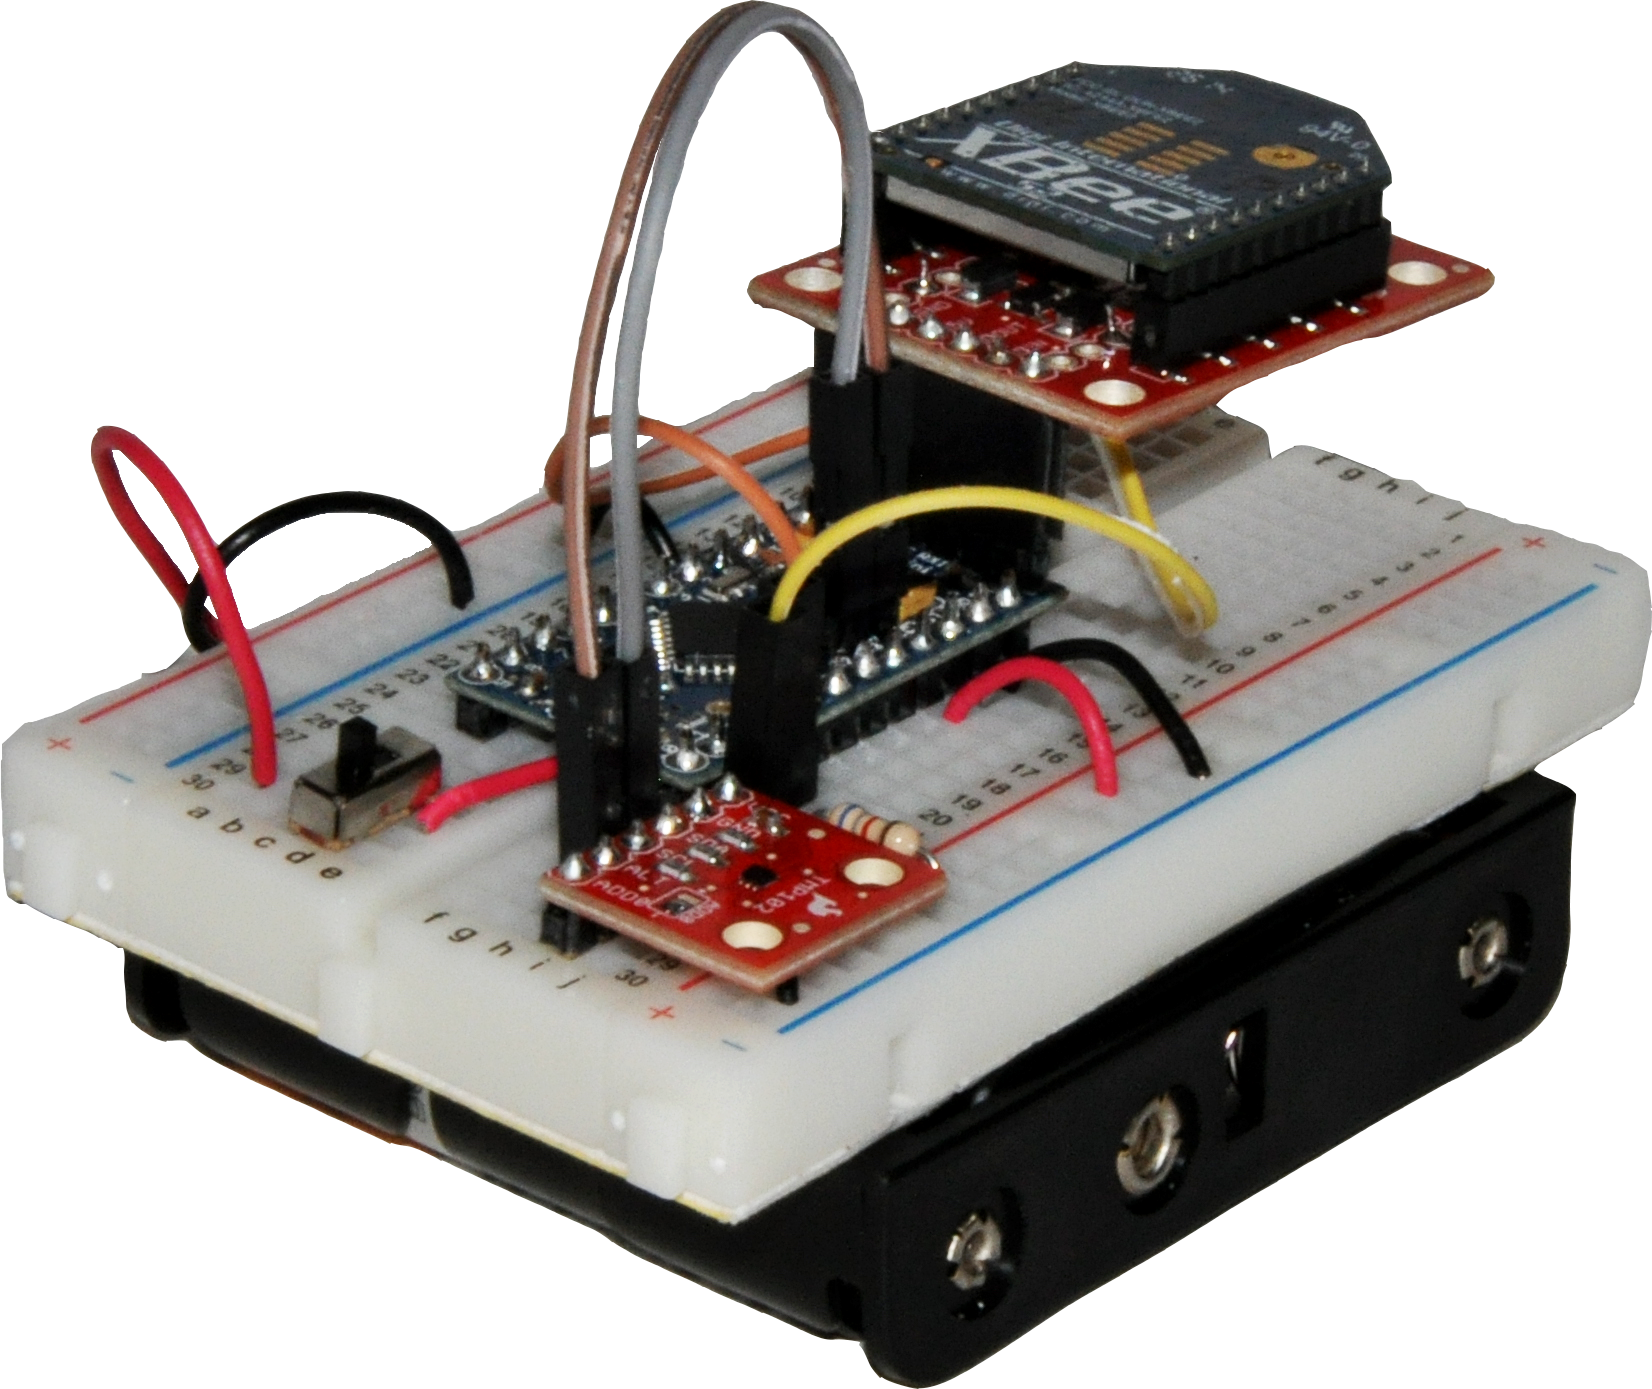
\includegraphics[width=0.6\textwidth]{assets/temp-prototype.png}};
          \end{tikzpicture}
        \caption{Prototype temperature device}\label{figure:temp-device}
      \end{figure}

      \begin{figure}
        \centering
          \begin{tikzpicture}
            \node[inner sep=0pt] at (0,0)
              {\includegraphics[width=0.8\textwidth]{assets/led-prototype.png}};
          \end{tikzpicture}
        \caption{Prototype RGB LED output device}\label{figure:led-device}
      \end{figure}

    \subsection{Energy Efficiency}
      One of the main concerns for the battery-powered devices was the battery life. In order for the application of devices to be practical, the batteries must not require constant charging or changing. Each device has two microcontroller units---the Arduino and the XBee radio chip. Both of these microcontrollers support various sleep modes, so these were employed to conserve energy.

      The deepest sleep mode available to the Arduino was implemented. Once the Arduino enters this deep sleep, it can only be awoken with an interrupt signal. For cyclic sensor devices which send a reading at regular intervals (temperature and RGB colour), the watchdog timer interrupt was used. This allows the Arduino to wake up after a pre-set length of time which is stored in the Watchdog Control Register.

      The watchdog timer technique was not appropriate for use with the gyroscope sensor. Data from the gyroscope sensor should be sent whenever motion is detected rather than at a set interval. The gyroscope sensor chip provides a hardware interrupt line extactly for this purpose. When motion is detected, the hardware interrupt is triggered and the Arduino is awoken from its deep sleep.

      An attempt was made to implement a hardware-based sleep mode with the XBee radio chips too. One of the XBee sleep modes allows the DTR (data ready) pin to be used as a hibernation pin; when it is brought high (3.3v) the XBee will enter a deep sleep and when it is brought low (0v), it will wake up. This technique uses a pull-up resistor to bring the DTR pin high by default and then relies on the Arduino sinking the current when it wants the XBee chip to wake up. The operation of this was sporadically unsuccessful and the root cause of the problem could not be identified. As a result, this feature was left out with the acknowledgement that more battery power will be consumed.

    \subsection{Data Transmission}
    \label{section:data-transmission}
      The Arduino board communicates with the XBee chip using a serial communication channel and there are a number of implementation details to discuss. First of all, the XBee can operate in two modes: transparent or API. With transparent mode, the XBee chip simply emulates a wired serial link whereas the API mode allows more advanced features to be used. API mode was chosen for this project due to the extra features it provides.

      Secondly, the end goal of the Haar Nodes is to interface with the Haar API. In order to do that, the sensed data must be communicated to the API. A common data-interchange format is required so that both the devices and the API are compatible. Arguably, the choice of format should belong in the design chapter, however it is dependent on the implementation of the Haar Engine APIs and models. Four different formats were considered: comma-separated value (CSV), JSON DB Schema, Compressed JSON DB Schema and Compressed JSON Map.

      Each of the formats have been described and explained below and there were a number of aims to satisfy. Firstly, size of data transmitted has an effect on power usage. More data means that the XBee chip has to transmit for longer periods, consuming battery power. The maximum packet size of an XBee transmission is 72 bytes \citep{xbee-packet-size}. In order to limit transmission to one packet, data size should aim to be less that this limit. Additionally, the format chosen should be robust and make it simple to distinguish the datapoints collected.\\

      \noindent
      \begin{minipage}[t]{0.45\textwidth}
        \textbf{Comma-separated value}\\
        The first data format explored was a simple comma-separated string. This created the smallest payload size (11 bytes for the given example).\\

        This format is not flexible, however. It requires the datapoints to maintain strict order, and requires all devices to know what this order is. The CSV string does not describe its contents at all - a developer would have no indication what the data refers to.\\
      \end{minipage}
      \hfill
      \begin{minipage}[t]{0.45\textwidth}
        \begin{lstlisting}[frame=single]
  123,123,123
        \end{lstlisting}
      \end{minipage}

      \noindent
      \begin{minipage}[t]{0.45\textwidth}
        \textbf{JSON DB Schema}\\
        The second format explored replicates the format of the Data Mongoose model used in the Haar Engine. Haar Engine explicitly defines `name' and `value' properties for use in validation. The size of the given example is 76 bytes, more than the 72 byte limit.\\

        This is the most descriptive format and requires no extra transformation before being sent to the Haar API. However, it is unsuitable because of its payload size.
      \end{minipage}
      \hfill
      \begin{minipage}[t]{0.45\textwidth}
        \begin{lstlisting}[frame=single]
  [
    {
      "name": "x",
      "value": 123
    },
    {
      "name": "y",
      "value": 123
    },
    {
      "name": "z",
      "value": 123
    }
  ]
        \end{lstlisting}
      \end{minipage}

      \noindent
      \begin{minipage}[t]{0.45\textwidth}
        \textbf{Compressed JSON DB Schema}\\
        Whilst investigating the previous format, it became apparent that it was unnecessarily expanding on the syntax of a JSON object. By their very nature, they are a key-value store. This means that the format can be condensed into the shown example (36 bytes).\\

        This format is both machine and human readable. Additionally, it does not require much additional trasformation in order to be submitted to the Haar API.\\
      \end{minipage}
      \hfill
      \begin{minipage}[t]{0.45\textwidth}
        \begin{lstlisting}[frame=single]
  [
    {
      "x": 123
    },
    {
      "y": 123
    },
    {
      "z": 123
    }
  ]
        \end{lstlisting}
      \end{minipage}

      \noindent
      \begin{minipage}[t]{0.45\textwidth}
        \textbf{Compressed JSON Object}\\
        Looking at the previous example, it is clear that there is a redundant structure in place. This format compresses the datapoints into a single JSON object, rather than an array with multiple nested objects. This yields an example payload size of 25 bytes.\\

        No information is lost between this format and the full JSON DB Schema option, meaning that it can be expanded to be successfully submitted to the Haar API and pass validation rules. This is the most effective format and has been chosen for use in the Haar Nodes. 
      \end{minipage}
      \hfill
      \begin{minipage}[t]{0.45\textwidth}
        \begin{lstlisting}[frame=single]
  {
    "x": 123,
    "y": 123,
    "z": 123
  }
        \end{lstlisting}
      \end{minipage}

      Figures \ref{figure:temp-device} and \ref{figure:led-device} show the finished prototype hardware for the temperature sensor and RGB LED actuator. The RGB colour and gyroscope sensors are similar to the temperature sensor. 

    \subsection{Testing}
      The constrained nature of this component required a different approach to testing. There were two main debugging methods used to assert correct operation for the Arduino boards: feedback messages via serial communication and simple signalling using the onboard LED. The programs for these devices were also simple, so they could be tested in a linear, start-to-finish fashion.

      The Arduino boards were connected with USB to a host computer for program compilation. Using this same USB connection it is possible to monitor serial transmissions from the Arduino board. Print statements were used at breakpoints in the program to inspect variable values and this was helpful when asserting the correct operation of sensor chips. The onboard LED was used as a simple flag and was especially useful when debugging Arduino sleep cycles. For example, when the board was awake the LED would be on and when the Arduino was put to sleep, the LED would be turned off.

      The final component which required testing was the XBee radio chip. The wiring used to connect the XBee to the Arduino used the FTDI (data communication) interface which is normally used by the USB connection when programming. This meant that serial communication of the Arduino could not be monitored. Instead, an additional XBee radio chip was connected to a computer using a breakout board which exposes USB. Software provided by the manufacturer called Digi XCTU was then used to monitor and interrogate transmission packets.   

  \section{Haar Bridge}
    The final and crucial component of the demonstration application is Haar Bridge. This component acts like a router; it translates the ZigBee-based packets of the Wireless Sensor Network into TCP/IP packets compatible with the wider Internet. In fact, Haar Bridge performs a bit more than simple translation---it also expands the data packet from the format discussed in Section \ref{section:data-transmission} into an API-compatible format. This brief section will discuss the hardware implementation as well as details of the software implementation.

    \subsection{Hardware}
      The hardware implementation made use of an Raspberry Pi model B+ (RPiB+) instead of the RPi2 as discussed in the design. The main reason for this was price; the RPiB+ was cheaper than the RPi2. The RPiB+ has a single-core 700MHz processor and 512MB RAM compared to a quad-core 900MHz processor and 1GB RAM, but it is still suffiently powerful for this project. When sourcing the RPi devices an additional component, the RPi Hardware on Top (HAT) prototype board, was found. Rather than connecting the RPi to the XBee chip with simple wires, this prototype board was used to build a more professional prototype.

      The RPi HAT is a semi-permanent board so unlike the breadboards used for the Arduino devices, some soldering was required to build the device. To ensure that the components were reusable for future projects, female pin headers were soldered onto the HAT so the XBee breakout board could be added or removed if necessary. The resulting form factor is quite pleasing and is shown in Figure \ref{figure:bridge-device}.

      \begin{figure}
        \centering
          \begin{tikzpicture}
            \node[inner sep=0pt] at (0,0)
              {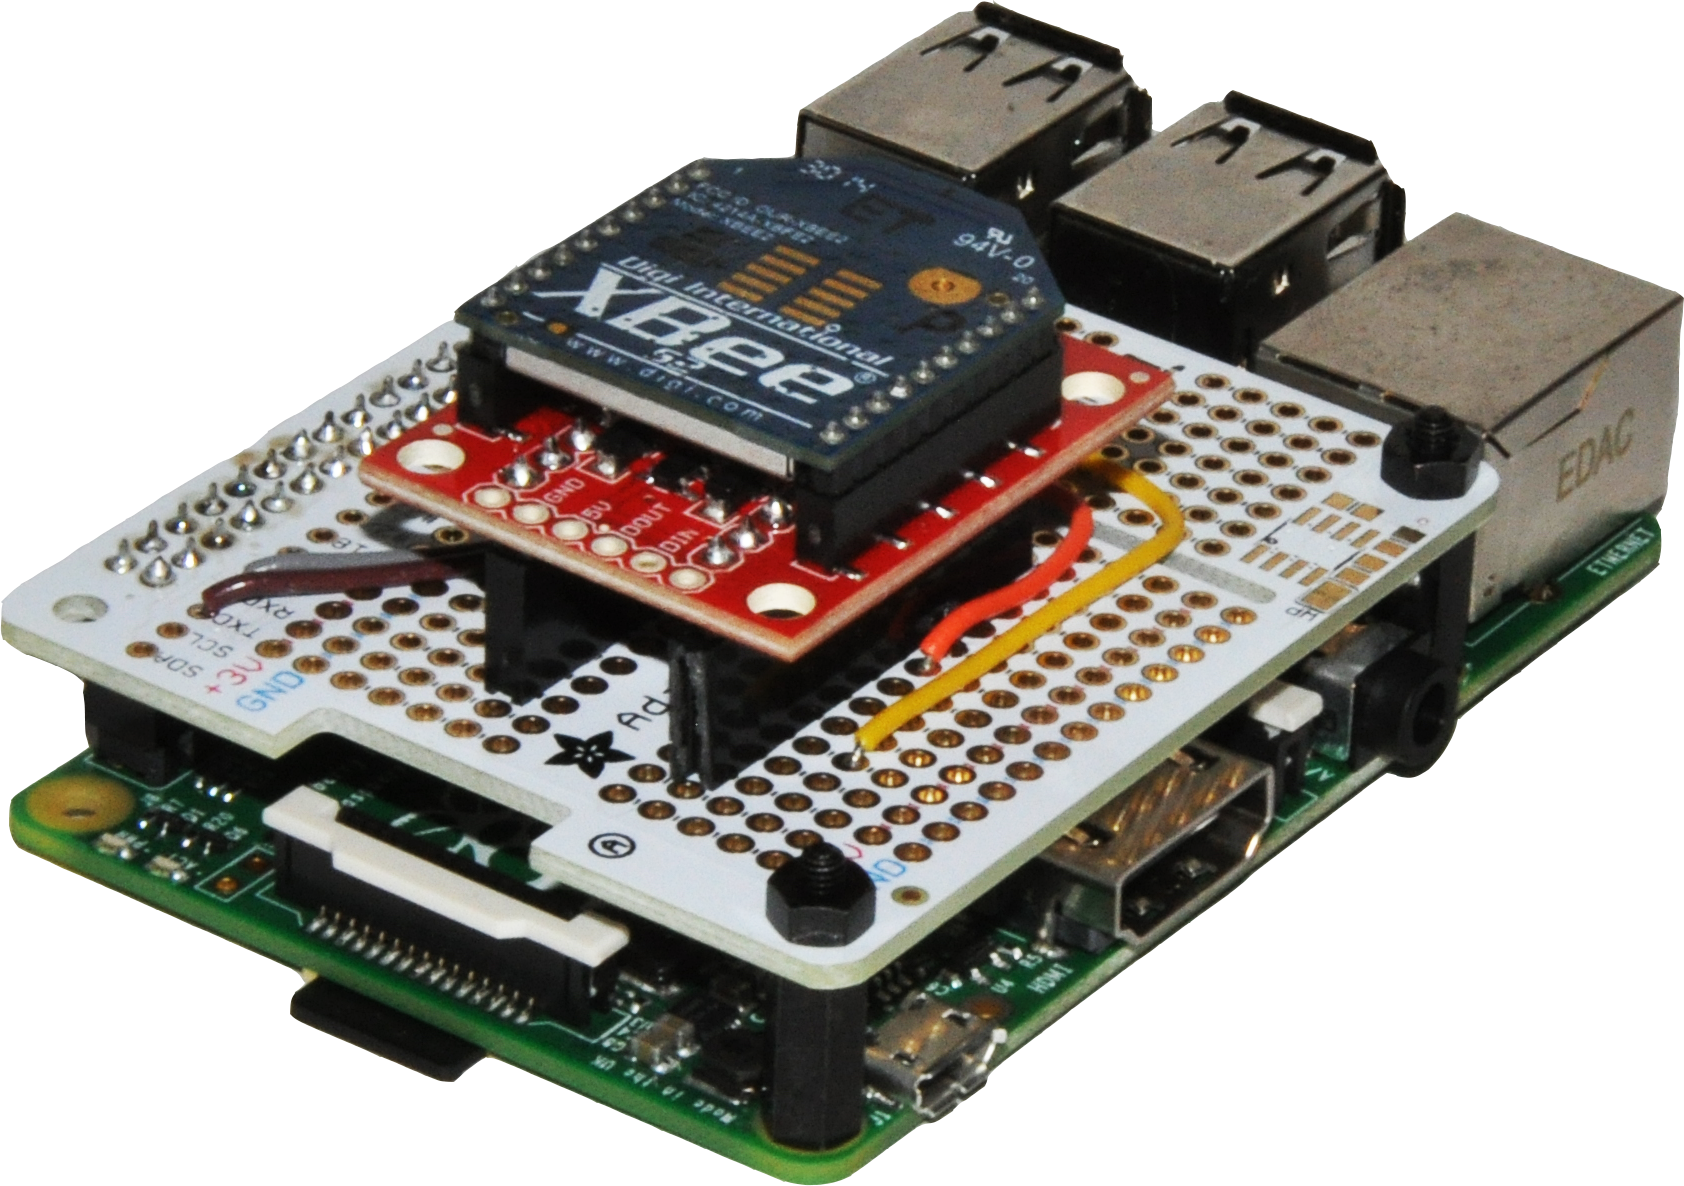
\includegraphics[width=0.6\textwidth]{assets/bridge-prototype.png}};
          \end{tikzpicture}
        \caption{Prototype bridge device}\label{figure:bridge-device}
      \end{figure}

    \subsection{Software}
      As planned, the RPi-maintained distribution of Linux was installed on the RPiB+. This gave a foundation for Haar Bridge software which, like the other Haar components, was developed as a Node.js application. This application used some of the same JavaScript packages which were implemented in the Haar Engine and Dashboard. There are two main functions which Haar Bridge must perform in order to operate correctly, namely: maintain a WebSocket connection with Haar API and maintain a serial connection with the XBee radio chip. These two functions are intertwined.

      Haar Bridge uses the Primus JavaScript package to open and maintain a single WebSocket connection. There are two stages in negotiating this WebSocket connection: user authentication and then topic subscription. When the application is started, an HTTP request is made to the Data Access API in order to retrieve a JWT token. The WebSocket connection is then initiated using this token. Once the WebSocket has been opened, the application can then subscribe to any appropriate event streams based on which devices it is connected to.

      Haar Bridge also uses the serialport and xbee-api JavaScript packages to maintain and parse serial communication between itself and the XBee radio chip. In order to support serial connections, the Raspberry Pi must first be configured to use its GPIO pins for a serial interface. The XBee radio chip and the Raspberry Pi support hardware flow control using clear-to-send (CTS) and request-to-send (RTS) pins. They are however not compatible and so hardware flow control was no implemented as designed.

      Once the WebSocket and serial communication channels were established, Haar Bridge could then perform its routing duties. If a WebSocket message is received, its contents will be forwarded to the appropriate ZigBee device. Conversely, if a serial message is received, it will be parsed by the xbee-api package. The data format will be expanded (as described in Figure \ref{figure:bridge-device}) and then a WebSocket message will be sent.

    \subsection{Testing}
      % Manual
        % XCTU
        % JS console.log statements     
